\let\negmedspace\undefined
\let\negthickspace\undefined
\documentclass[journal]{IEEEtran}
\usepackage[a5paper, margin=10mm, onecolumn]{geometry}
%\usepackage{lmodern} % Ensure lmodern is loaded for pdflatex
\usepackage{tfrupee} % Include tfrupee package

\setlength{\headheight}{1cm} % Set the height of the header box
\setlength{\headsep}{0mm}     % Set the distance between the header box and the top of the text

\usepackage{gvv-book}
\usepackage{gvv}
\usepackage{cite}
\usepackage{amsmath,amssymb,amsfonts,amsthm}
\usepackage{algorithmic}
\usepackage{graphicx}
\usepackage{textcomp}
\usepackage{xcolor}
\usepackage{txfonts}
\usepackage{listings}
\usepackage{enumitem}
\usepackage{mathtools}
\usepackage{gensymb}
\usepackage{comment}
\usepackage[breaklinks=true]{hyperref}
\usepackage{tkz-euclide} 
\usepackage{listings}
\usepackage{gvv}                                        
\def\inputGnumericTable{}                                 
\usepackage[latin1]{inputenc}                                
\usepackage{color}                                            
\usepackage{array}                                            
\usepackage{longtable}                                       
\usepackage{calc}                                             
\usepackage{multirow}                                         
\usepackage{hhline}                                           
\usepackage{ifthen}                                           
\usepackage{lscape}
\usepackage{circuitikz}
\tikzstyle{block} = [rectangle, draw, fill=blue!20, 
    text width=4em, text centered, rounded corners, minimum height=3em]
\tikzstyle{sum} = [draw, fill=blue!10, circle, minimum size=1cm, node distance=1.5cm]
\tikzstyle{input} = [coordinate]
\tikzstyle{output} = [coordinate]

\begin{document}


\bibliographystyle{IEEEtran}
\vspace{3cm}

\title{4.11.26}
\author{EE25BTECH11049 - Sai Krishna Bakki}
 \maketitle
% \newpage
% \bigskip
{\let\newpage\relax\maketitle}

\renewcommand{\thefigure}{\theenumi}
\renewcommand{\thetable}{\theenumi}
\setlength{\intextsep}{10pt} % Space between text and floats


\numberwithin{equation}{enumi}
\numberwithin{figure}{enumi}
\renewcommand{\thetable}{\theenumi}
\textbf{Question:}\\
Find the area bounded by the curves $y = |x - 1|$ and $y = 1$.\\
\textbf{Solution}
\subsection*{1. Representing Lines in Matrix Form}
We express the three boundary lines in the vector form $\vec{n}^T \vec{x} = c$, where $\vec{n}$ is the normal vector and $\vec{x} = \myvec{x \\ y}$.
\begin{align}
    \vec{n_1}=\myvec{1\\-1},c_1=1\implies \myvec{1 & -1}\vec{x}=1\\
    \vec{n_2}=\myvec{1\\1},c_1=1\implies \myvec{1 & 1}\vec{x}=1\\
    \vec{n_3}=\myvec{0\\1},c_1=1\implies \myvec{0 &1}\vec{x}=1
\end{align}

\subsection*{2. Finding Vertices with Matrix Inversion}
The intersection of any two lines is the solution to a system of linear equations, which we solve using matrix inversion.

\subsubsection*{Vertex A (Intersection of $L_1$ and $L_2$)}
The system is $\myvec{1 & -1 \\ 1 & 1} \myvec{x \\ y} = \myvec{1 \\ 1}$. The solution is $\vec{x} = \vec{N}_{12}^{-1}\vec{c}_{12}$.
\begin{align}  
\vec{A} &= \myvec{1 & -1 \\ 1 & 1}^{-1} \myvec{1 \\ 1} \\
&= \frac{1}{1(1) - (-1)(1)} \myvec{1 & 1 \\ -1 & 1} \myvec{1 \\ 1} \\
&= \frac{1}{2} \myvec{1(1) + 1(1) \\ -1(1) + 1(1)} = \frac{1}{2} \myvec{2 \\ 0} = \myvec{1 \\ 0}
\end{align}  

\subsubsection*{Vertex B (Intersection of $L_1$ and $L_3$)}
The system is $\myvec{1 & -1 \\ 0 & 1} \myvec{x \\ y} = \myvec{1 \\ 1}$. The solution is $\vec{x} = \vec{N}_{13}^{-1}\vec{c}_{13}$.
\begin{align}  
\vec{B} &= \myvec{1 & -1 \\ 0 & 1}^{-1} \myvec{1 \\ 1} \\
&= \frac{1}{1(1) - (-1)(0)} \myvec{1 & 1 \\ 0 & 1} \myvec{1 \\ 1} \\
&= \myvec{1(1) + 1(1) \\ 0(1) + 1(1)} = \myvec{2 \\ 1}
\end{align}  

\subsubsection*{Vertex C (Intersection of $L_2$ and $L_3$)}
The system is $\myvec{1 & 1 \\ 0 & 1} \myvec{x \\ y} = \myvec{1 \\ 1}$. The solution is $\vec{x} = \vec{N}_{23}^{-1}\vec{c}_{23}$.
\begin{align}  
\vec{C} &= \myvec{1 & 1 \\ 0 & 1}^{-1} \myvec{1 \\ 1} \\
&= \frac{1}{1(1) - 1(0)} \myvec{1 & -1 \\ 0 & 1} \myvec{1 \\ 1} \\
&= \myvec{1(1) - 1(1) \\ 0(1) + 1(1)} = \myvec{0 \\ 1}
\end{align}  
The vertices are $\vec{A}=(1,0)$, $\vec{B}=(2,1)$, and $\vec{C}=(0,1)$.

\subsection*{3. Calculating Area with Vector Determinant}
We form two vectors representing two sides of the triangle, $\vec{AB}$ and $\vec{AC}$.
\begin{align}  
\vec{AB} &= \vec{B} - \vec{A} = \myvec{2 \\ 1} - \myvec{1 \\ 0} = \myvec{1 \\ 1} \\
\vec{AC} &= \vec{C} - \vec{A} = \myvec{0 \\ 1} - \myvec{1 \\ 0} = \myvec{-1 \\ 1}
\end{align}  
The area is half the absolute value of the determinant of the matrix formed by these two vectors.
\begin{align}  
\text{Area} &=\frac{1}{2}\abs{\mydet{\myvec{{\vec{B}-\vec{A}}}\times{\vec{C}-\vec{A}}}} \\
\text{Area} &= \frac{1}{2} \abs{\mydet{1 & -1 \\ 1 & 1}} \\
&= \frac{1}{2} \brak{1(1) - (-1)(1)} \\
&= \frac{1}{2} \brak{1 + 1} = \frac{1}{2} \brak{2} = 1 \text{ square unit.}
\end{align}  
\newpage
 \begin{figure}
    \centering
    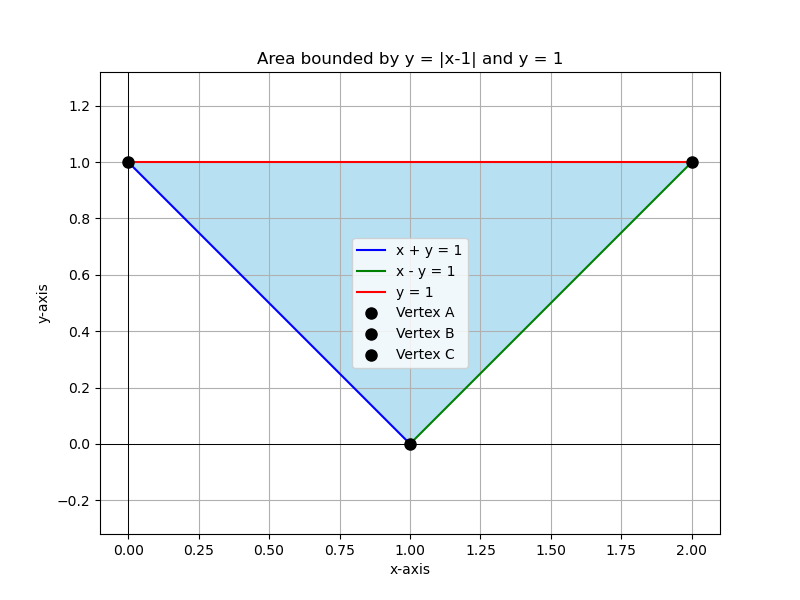
\includegraphics[width=0.9\columnwidth]{figs/Figure_1.png}
    \label{fig:placeholder}
    \caption{}
\end{figure}

\end{document}